% !TeX root = er.tex

\chapter{Units of measurement}\label{ch.units}
\index{units of measurement}

Tables~\ref{tab.units} and \ref{tab.prefixes} show the units of measurement and their abbreviations.

\begin{table}
\caption{Units of measurement}
\label{tab.units}
\begin{tabular}{p{2cm}p{1.5cm}p{2.5cm}p{2cm}}
\svhline\noalign{\smallskip}
Property & Variable & Unit & Abbreviation \\
\noalign{\smallskip}\svhline\noalign{\smallskip}
Distance & $s$ & meter  & m\\
Time &  $t$ & second & s\\
Velocity & $v$ & meter/second &  m/s\\
Acceleration & $a$ & meter/second$^2$ & m/s$^2$\\
Frequency & $f$ & hertz & Hz\\
Angle & $\theta$ & radian & rad\\
& & degree & $^\circ$\\
\noalign{\smallskip}\svhline\noalign{\smallskip}
\end{tabular}
\end{table}

\begin{table}
\caption{Prefixes}
\label{tab.prefixes}
\begin{tabular}{p{1.5cm}p{2.2cm}p{1.7cm}}
\svhline\noalign{\smallskip}
Prefix & Meaning & Abbreviation \\
\noalign{\smallskip}\svhline\noalign{\smallskip}
kilo- & thousands & k\\
centi- & hundreths & c\\
milli- & thousandths & m\\
micro- & millionths & $\mu$\\
\noalign{\smallskip}\svhline\noalign{\smallskip}
\end{tabular}
\end{table}

\noindent\textbf{Examples:}

\begin{itemize}\setlength{\itemsep}{6pt}
\item $20$ kHz $=$ $20$ kilohertz $=$ $20,000$ hertz
\item $15$ cm $=$ $15$ centimeters $=$ $\frac{15}{100}$ meters
\item $50$ ms $=$ $50$ milliseconds $=$ $\frac{50}{1000}$ seconds
\item $10$ $\mu$s $=$ $10$ microseconds $=$ $\frac{10}{1000}$ milliseconds $=$ $\frac{10}{1000000}$ seconds
\end{itemize}

Angles, such as the heading of a robot and the direction to an object, are measured in degrees or radians (Fig.~\ref{fig.angles}). By convention, angles are positive in the counterclockwise direction and negative in the clockwise direction as measured from the front of the robot.

\begin{figure}
\begin{center}
% The unit circle divided into 45 degree segments
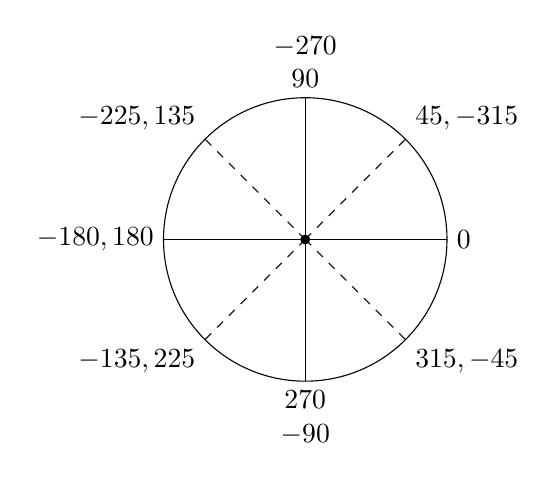
\begin{tikzpicture}[scale=1.8]
\coordinate (origin) at (0,0);
% Draw circle
\draw (origin) circle [radius=1];
% Draw axes
\draw (-1,0) node [left] {$-180,180$} -- (1,0) node [right] {$0$};
\draw (0,-1) node [below,align=flush center] {$270$\\$-90$} -- (0,1) node [above,align=flush center] {$-270$\\$90$};
% Draw other angles
\draw[dashed] (origin) -- +(45:1) node[above right] {$45,-315$};
\draw[dashed] (origin) -- +(135:1) node[above left] {$-225,135$};
\draw[dashed] (origin) -- +(225:1) node[below left] {$-135,225$};
\draw[dashed] (origin) -- +(315:1) node[below right] {$315,-45$};
% Dot at origin
\fill (origin) circle [radius=1pt];
\end{tikzpicture}
\hspace{\fill}
% The unit circle with radians divided into pi/4 segments
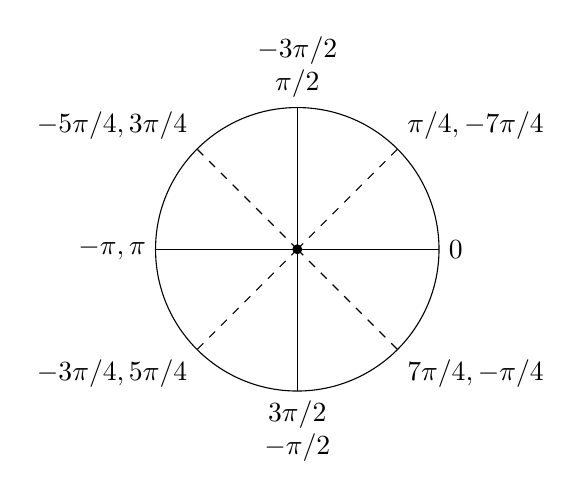
\begin{tikzpicture}[scale=1.8]
\coordinate (origin) at (0,0);
% Draw circle
\draw (origin) circle [radius=1];
% Draw axes
\draw (-1,0) node [left] {$-\pi,\pi$} -- (1,0) node [right] {$0$};
\draw (0,-1) node [below,align=flush center] {$3\pi/2$\\$-\pi/2$} -- (0,1) node [above,align=flush center] {$-3\pi/2$\\$\pi/2$};
% Draw other angles
\draw[dashed] (origin) -- +(45:1) node[above right] {$\pi/4,-7\pi/4$};
\draw[dashed] (origin) -- +(135:1) node[above left] {$-5\pi/4,3\pi/4$};
\draw[dashed] (origin) -- +(225:1) node[below left] {$-3\pi/4,5\pi/4$};
\draw[dashed] (origin) -- +(315:1) node[below right] {$7\pi/4,-\pi/4$};
% Dot at origin
\fill (origin) circle [radius=1pt];
\end{tikzpicture}
\end{center}
\caption{Angles in degrees (left) and radians (right)}\label{fig.angles}
\end{figure}

\chapter{Mathematical derivations and tutorials}\label{ch.math}

This appendix collects mathematical derivations used in the text as well as short tutorials of concepts which may not be familiar.

\section{Conditional probability and Bayes rule}\label{a.bayes}

Given a reading $z$ of the sensor, what is the probability that we are at position $x_i$? This is expressed as a \emph{conditional probability}\index{probability!conditional} $p(x_i\mid z)$. The data we have available are the \emph{current} probability $p(x_i)$ that we are at $x_i$, and $p(z\mid x_i)$, the conditional probability that the sensor reads $z$ if we are in fact at $x_i$. Let us multiply these two probabilities:
\[
p(z\mid x_i)\, p(x_i)\,.
\]
What does this mean? The event $x_i$ occurs with probability $p(x_i)$ and once it occurs the event $z$ occurs with probability $p(z\mid x_i)$. Therefore, this is the probability that both $z$ and $x_i$ occur, called the \emph{joint	probability}\index{probability!joint} of the two events:
\[
p(z \cap x_i) = p(z\mid x_i)\, p(x_i)\,.
\]
The joint probability can also be obtained by multiplying the conditional probability for $x_i$ given $z$ by the probability of $z$:
\[
p(x_i \cap z) = p(x_i\mid z)\, p(z)\,.
\]
The joint probability is commutative so by equating the two expressions we have:
\[
p(x_i\mid z)\, p(z) = p(x_i \cap z) = p(z \cap x_i) = p(z\mid x_i)\, p(x_i)\,.
\]
Dividing by $p(z)$ gives:
\[
p(x_i\mid z)= \frac{p(z\mid x_i)\, p(x_i)}{p(z)}\,,
\]
which is known as \emph{Bayes rule}\index{probability!Bayes rule}.

If we know $p(z\mid x_i)$ and $p(x_i)$ for each $i$, $p(z)$, the \emph{total probability} of the event $z$, can be computed by summing the individual known probabilities:
\begin{displaymath}
p(z) = \sum_i p(z\mid x_i)\, p(x_i)\,.
\end{displaymath}

\noindent\textbf{Example} Let us do the computation for the example in Sect.~\ref{s.prob-local}. Let $x_i$ be the event that we are at position $i$ and let $z$ be the event that the robot detects a door. Initially, $p(x_i)=.125$ for all positions $x_i$, and, if the robot is at a door, the probability that the sensor detects this correctly is $.9$, while the probability that it incorrectly detects a door is $1-.9=.1$. The probability of detecting a door, $p(z)$, is obtained by summing the probabilities at each position, where the probability is $.125\times 0.9 = .1125$ at a position with a door and $.125\times .1= .0125$ at a position with no door:
\[
p(z)=.1125 + .1125 + .0125 + .0125 + .1125 + .1125 + .1125 + .0125 = .575\,.
\]
By Bayes rule, the probability of being at position $i$ with a door \emph{if} a door is detected is:
\[
p(x_i \mid z) = \frac{p(z\mid x_i)\, p(x_i)}{p(z)}=\frac{.9\times .125}{.575} = .196\,,
\]
while the probability of being at position $i$ with no door, but incorrectly a door is detected is:
\[
p(x_i \mid z) = \frac{p(z\mid x_i)\, p(x_i)}{p(z)}=\frac{.1\times .125}{.575} = .022\,.
\]

\section{Normalization}\label{a.normalize}
\index{probability!normalization}

The set of probabilities of the possible outcomes of an event must add up to $1$ since one of the outcomes must occur. If a door is detected, the robot must be at one of the $8$ possible positions, but the sum over all positions $i$ of the probability that the robot is at position $i$ was shown above to be:
\[
.1125 + .1125 + .0125 + .0125 + .1125 + .1125 + .1125 + .0125 = .575\,.
\]
The probabilities must be \emph{normalized} by dividing by the sum $.575$ so that the sum will be $1$. The normalized probabilities are $.1125/.575\approx .19$ and  $.0125/.575\approx .02$, which do add up to $1$:
\[.19 + .19 + .02 + .02 + .19 + .19 + .19 + .02 \approx 1\,.\]

\section{Mean and variance}\label{a.mean}

The \emph{mean}\index{probability!mean}\footnote{\textit{Mean} is the technical term for average.} $\mu$ of a set of values $\{x_1,\ldots,x_n\}$ is:
\[
\mu = \frac{1}{n}\sum^n_{i=1} x_i\,.
\]
Consider five people earning $8,9,10,11,12$ thousand Euros per year, respectively. Their mean salary is:
\[
\mu = \frac{8+9+10+11+12}{5} = \frac{50}{5} = 10\,.
\]
The mean doesn't tell us very much because the same mean can be obtained from very different data:
\[
\mu = \frac{5+6+10+14+15}{5} = \frac{50}{5} = 10\,.
\]
The mean is significantly influenced by \emph{outliers}: values that are much higher or lower than the rest of the values. If the person earning $10$ thousand Euros suddenly received a bonus of $90$ thousand Euros, the mean salary is now:
\[
\mu = \frac{8+9+100+11+12}{5} = \frac{140}{5} = 28\,.
\]
A politician would jump at the opportunity of claiming that during his term of office the average salary had risen by $180\%$!

\emph{Variance}\index{probability!variance} is a measure of the spread of a set of values. The closer together the values are, the lower the variance. Measures like the mean are more reliable if the values are clustered together and thus have a low variance. The formula for the variance of a set of values $\{x_1,\ldots,x_n\}$ is:\footnote{$n-1$ counts the \emph{degrees of freedom}. Since the mean is computed before the variance, we can't choose the $n$ values arbitrarily; the last value chosen is constrained to be the value that causes the computation to produce the given mean.}
\[
s^2 = \frac{1}{n-1}\sum^n_{i=1} (x_i-\mu)^2\,.
\]
Each term $x_i-\mu$ measures the distance of the value $x_i$ from the mean; the variance is the average of the squares of these distances. The distances are squared so that values on either side of the mean don't cancel each other out. For example, given values $100$ and $300$, their mean is $200$; if we computed the variance as $(100-200)+(200-300)$, the result would be $0$ even though the values are spread out. Using the definition above, the variance is $(100-200)^2+(200-300)^2=20000$.

For the data set $\{8,9,10,11,12\}$ the variance is:
\[
s^2 = \frac{(-2)^2+(-1)^2+0+1^2+2^2}{5-1} = \frac{10}{4} = 2.5\,,
\]
while for the data set $\{5,6,10,14,15\}$ the variance is:
\[
s^2 = \frac{(-5)^2+(-4)^2+0+4^2+5^2}{4} = 20.5\,.
\]
Since $20.5$ is much larger than $2.5$ the data in the second set are spread over a wider range than the data of the first set. After the bonus is received the variance is:
\[
s^2 = \frac{20^2+19^2+72^2+17^2+16^2}{4} = \frac{6490}{4} = 1622.5\,.
\]
Clearly, one shouldn't interpret the mean salary as meaningful if there are outliers.

\section{Covariance}\label{a.covariance}
\index{probability!covariance}

Consider a group of ten people earning the following salaries:
\[x_1=\{11,12,13,14,15,16,17,18,19,20\}\,,
\]
in thousands of Euros. The average salary is:
\[
\mu_1=\frac{1}{10}(11+12+13+14+15+16+17+18+19+20)=15.5\,.
\]
We conjecture that people with higher salaries buy more expensive cars than those with low salaries. Suppose that there are two models of cars being sold in that area, one for $10$ thousand Euros and one for $20$ thousand Euros. The following data set shows the cars bought by this group of people, where the $i$'th element is the cost of the car bought by the $i$'th person:
\[
x_2=\{10,10,10,20,10,20,10,10,20,20\}\,.
\]
To see if there is any connection between the salaries and the costs of the cars, the \emph{covariance} $\textit{cov}(x_1,x_2)$ between the data sets $x_1$ and $x_2$ is calculated. The computation is similar to that of the variance, except that instead of squaring the difference between a value in a single set and the mean of that set, we multiply the difference between a value from the first set and its mean by the difference between a value from the second set and its mean:
\[
\textit{cov}(x_1,x_2) = \frac{1}{n-1}\sum^n_{i=1} (x_{1,i}-\mu_1)(x_{2,i}-\mu_2)\,.\label{eq.cov}
\]
The covariance of the sets of value $x_1$ and $x_2$ is $7.8$, a positive value, which indicates that salaries and car cost increase together, that is, people making more money tend to buy more expensive cars. If the first five people buy cars worth $10$ and the next five people buy cars worth $20$, the covariance becomes $13.9$, indicating a stronger connection between salary and the cost of a car. Conversely, if the first five buy expensive cars and the next five buy cheap cars, the covariance is $-13.9$, so that as the salary goes up, the cost of a car goes down. Finally, if everyone buys the same car, the covariance is $0$ and we conclude as expected that there is no connection between one's salary and the car one buys.

Covariance is symmetric because multiplication of real numbers is commutative:
\begin{eqnarray*}
\textit{cov}(x_1,x_2) &=& \frac{1}{n-1}\sum^n_{i=1} (x_{1,i}-\mu_1)(x_{2,i}-\mu_2)\\
&=& \frac{1}{n-1}\sum^n_{i=1} (x_{2,i}-\mu_2)(x_{1,i}-\mu_1)\\
&=&\textit{cov}(x_2,x_1)\,.
\end{eqnarray*}

The covariance matrix combines the variances and the covariances:
\[
\left[ \begin{array}{ll} s^2(x_1) & \textit{cov}(x_1,x_2)\\ \textit{cov}(x_2,x_1)& s^2(x_2)\end{array}\right]\,.
\]
$\textit{cov}(x_1,x_2)=\textit{cov}(x_2,x_1)$, so there are only three different values in the matrix.

\section{Multiplication of vectors and matrices}\label{a.matrices}
\index{matrix multiplication}

Multiplication of a (two-dimensional) matrix $\vec{M}$ by a vector $\vec{v}$ gives a new vector:
\[
\spacearray
\vec{M}\vec{v}=\left[ \begin{array}{c} a\\c\end{array} \begin{array}{c} b\\d \end{array}\right]\, \left[ \begin{array}{c} x\\y\end{array}\right] = \left[ \begin{array}{c} ax+by\\cx+by\end{array}\right]\,.
\]
Multiplication of two matrices is performed by multiplying the rows of left matrix separately with each column vector of the right matrix to get the column vectors for the resulting matrix:
\[
\spacearray
\left[ \begin{array}{c} a\\c\end{array} \begin{array}{c} b\\d \end{array}\right]\, \left[ \begin{array}{c} x\\y\end{array} \begin{array}{c} u\\v\end{array}\right] = \left[ \begin{array}{c} ax+by\\cx+dy\end{array} \;\; \begin{array}{c} au+bv\\cu+dv\end{array}\right]\,.
\]
The identity matrix is:
\[
\spacearray
\vec{I}=\left[\begin{array}{c} 1\\0\end{array} \begin{array}{c} 0\\1\end{array}\right]
\]
and it is easy to check that for any matrix $\vec{M}$, $\vec{M}\, \vec{I} = \vec{I}\, \vec{M} = \vec{M}$.
For a matrix $\vec{M}$, its inverse $\vec{M}^{-1}$ is the matrix that results in $\vec{I}$ when multiplied by $\vec{M}$:
\[
\spacearray
\vec{M}=\left[ \begin{array}{c} a\\c\end{array} \begin{array}{c} b\\d \end{array}\right]\,,\;\;\;\;
\vec{M}^{-1}=\frac{1}{\textit{det}\,(\vec{M})}\left[ \begin{array}{c} d\\-c\end{array} \begin{array}{c} -b\\a \end{array}\right]\,,
\]
where $\textit{det}\,(\vec{M})$, the \emph{determinant} of $\vec{M}$, is $ad-bc$. We can check this by multiplying:
\[
\spacearray
\left[ \begin{array}{c} a\\c\end{array} \begin{array}{c} b\\d \end{array}\right] \cdot
\left[ \begin{array}{c} d\\-c\end{array} \begin{array}{c} -b\\a \end{array}\right] =
\left[ \begin{array}{c} ad-bc\\cd-dc\end{array} \;\;\begin{array}{c} -ab+ba\\-bc+da \end{array}\right] =
\left[ \begin{array}{c}ad-bc \\0\end{array}\;\; \begin{array}{c} 0\\ad-bc \end{array}\right]\,.
\]
This is valid only for matrices whose determinant is non-zero, because \emph{singular} matrices---those whose determinant is zero---do not have an inverse.


\section{The area of a trapezoid at the base of a triangle}\label{a.trap}
\index{trapezoid}

The following diagram shows a triangle of width $w$ and height $h$ with a parallel line at height $h'$ that creates a trapezoid:

\begin{center}
% Computing the area from the uncertainty
\begin{tikzpicture}[scale=1.3]
\draw (0,0) -- (1.5,3) -- (3,0) -- node[below] {$w$} cycle;
\draw (.5,1) -- node[below] {$w'$} (2.5,1);
\draw[<->] (-.4,0) -- node[left] {$h$} (-.4,3);
\draw[<->] (3.4,0) -- node[right] {$h'$} (3.4,1);
\draw[<->] (3.4,1) -- node[right] {$h-h'$} (3.4,3);
\end{tikzpicture}
\end{center}

We want to find a formula for the area of the trapezoid using the values $w, h, h'$. The area $a$ is the difference between the the areas of the two triangles:
\begin{displaymath}
a = \frac{wh}{2} - \frac{w'(h-h')}{2}\,.
\end{displaymath}
By similar triangles:
\begin{displaymath}
\frac{h}{h-h'} = \frac{w}{w'}\,,
\end{displaymath}
so:
\begin{displaymath}
w' = \frac{w(h-h')}{h}\,.
\end{displaymath}
Substituting:
\begin{eqnarray*}
a &=& \frac{wh}{2} - \frac{w(h-h')(h-h')}{2h}\\[8pt]
&=&\frac{w(h^2-(h-h')^2)}{2h}\\[8pt]
&=&\frac{w(h^2-h^2+2hh'-h'^2)}{2h}\\[8pt]
&=&\frac{w(2hh'-h'^2)}{2h}\\[8pt]
&=&wh'(1-\frac{h'}{2h})\,.
\end{eqnarray*}

\section{Algebraic formulas for $\cos 15^{\circ}$}\label{a.cosine}

Eq.~\ref{eq.cos15} claims that:
\[
\cos^{-1}\left(\frac{\sqrt{2+\sqrt{3}}}{2}\right) = \pm 15^{\circ}\,.
\]
Using the formula for the cosine of the difference of two angles, we have:
\begin{eqnarray*}
\cos 15^\circ &=& \cos(45^\circ-30^\circ)\\
&=& \cos 45^\circ \cos 30^\circ + \sin 45^\circ \sin 30^\circ\\
&=&\frac{\sqrt{2}}{2}\cdot \frac{1}{2} + \frac{\sqrt{2}}{2}\cdot \frac{\sqrt{3}}{2}\\
&=&\frac{\sqrt{2}+\sqrt{6}}{4}\,.
\end{eqnarray*}
We now compute:
\[
\left(\frac{\sqrt{2}+\sqrt{6}}{4}\right)^2 =
\left(\frac{8+2\sqrt{2}\sqrt{6}}{16}\right)=\frac{2+\sqrt{3}}{4}=
\left(\frac{\sqrt{2+\sqrt{3}}}{2}\right)^2\,.
\]
